\documentclass{article}
\usepackage[paperwidth=594mm,paperheight=841mm,top=13mm,bottom=12mm,left=14mm,right=14mm]{geometry}
\usepackage[T1]{fontenc}
\usepackage{helvet}
\usepackage{xcolor}
\usepackage{graphicx}
\usepackage{tcolorbox}
\usepackage{ragged2e}
\usepackage{array}
\usepackage{microtype}
\renewcommand{\familydefault}{\sfdefault}
\definecolor{paper}{HTML}{F7F4ED}
\definecolor{ink}{HTML}{17324D}
\definecolor{accent}{HTML}{D55E00}
\definecolor{blue}{HTML}{0072B2}
\definecolor{soft}{HTML}{EAE5DC}
\pagecolor{paper}
\color{ink}
\pagestyle{empty}
\setlength{\parindent}{0pt}
\setlength{\parskip}{4mm}
\hyphenpenalty=10000
\exhyphenpenalty=10000
\newcommand{\TargetAccuracy}{50.0\%}
\newcommand{\ContextAccuracy}{55.5\%}
\newcommand{\BertAccuracy}{67.1\%}
\newcommand{\AccuracyGain}{11.6}
\newcommand{\BertMacroF}{66.7\%}
\newcommand{\ContextMacroF}{55.1\%}
\newcommand{\DifferenceLower}{-16.9}
\newcommand{\DifferenceUpper}{-6.6}
\newcommand{\ValidationCount}{638}
\newcommand{\SelectionHash}{debfd61b068f22ea1a737f238bd90ea4fb8bf44f675907e428949b559a0bb309}
\newcommand{\BertOnlyCount}{178}
\newcommand{\StaticOnlyCount}{104}
\newcommand{\BertErrorCount}{210}

\newtcolorbox{panel}[1]{
  colback=white,colframe=soft,boxrule=0.8mm,arc=2mm,
  left=5mm,right=5mm,top=4mm,bottom=4mm,before skip=5mm,after skip=5mm,
  title={#1},coltitle=ink,fonttitle=\fontsize{32}{37}\selectfont\bfseries,
  halign title=left
}
\newcommand{\bodyfont}{\fontsize{28}{34}\selectfont}
\newcommand{\captionfont}{\fontsize{24}{29}\selectfont}
\newcommand{\tinyfooter}{\fontsize{15}{18}\selectfont}
\newcommand{\key}[1]{\textcolor{accent}{\bfseries #1}}
\begin{document}
\bodyfont
\begin{minipage}[t]{0.74\textwidth}
  {\fontsize{59}{63}\selectfont\bfseries A word is not one vector}\par
  \vspace{3mm}
  {\fontsize{31}{36}\selectfont Static vs contextual embeddings for lexical ambiguity on WiC}
\end{minipage}\hfill
\begin{minipage}[t]{0.23\textwidth}\RaggedLeft
  {\fontsize{25}{30}\selectfont\bfseries Student Name}\par
  {\fontsize{20}{24}\selectfont replace before submission}\par
  \vspace{5mm}
  {\fontsize{18}{22}\selectfont MSc Natural Language Processing\par
  Trends in Natural Language Processing}
\end{minipage}

\vspace{7mm}
\begin{tcolorbox}[colback=accent,colframe=accent,arc=2mm,boxrule=0pt,left=8mm,right=8mm,top=6mm,bottom=6mm]
\color{white}\centering
{\fontsize{42}{48}\selectfont\bfseries Frozen BERT adds \AccuracyGain{} accuracy points over local GloVe context}\par
{\fontsize{24}{29}\selectfont \BertAccuracy{} vs \ContextAccuracy{}; paired 95\% interval for GloVe minus BERT: [\DifferenceLower{}, \DifferenceUpper{}] points}
\end{tcolorbox}

\vspace{2mm}
\noindent
\begin{minipage}[t]{0.316\textwidth}
\RaggedRight
\begin{panel}{Hypothesis}
The same word form can express different meanings. A static target embedding
cannot react to that context; a contextual target embedding should place
same-sense occurrences closer together than different-sense occurrences.

\key{Prediction:} frozen BERT target similarity will separate WiC labels better
than either a context-free GloVe target or an average of nearby GloVe words.
\end{panel}

\begin{panel}{Methodology}
\textbf{Data.} Official SuperGLUE v2 WiC: 5,428 balanced training pairs and one
final evaluation on \ValidationCount{} balanced validation pairs. The 1,400-row
test split has no public labels and is not reported. [1]

\textbf{Static representations.} GloVe 6B 300d [2]: (i) the lemma vector on both
sides; (ii) mean in-vocabulary context vectors after excluding the marked target.
Candidate windows were $\pm2$, $\pm5$, $\pm10$, and sentence.

\textbf{Contextual representation.} Unfine-tuned BERT-base-uncased [3]. Fast
tokenizer offsets select every WordPiece overlapping the supplied half-open
character span; WordPieces are mean pooled. Candidates: final layer and mean of
the last four layers.

\textbf{Decision rule.} Cosine similarity $\geq$ a global threshold means
same-sense. Thresholds maximize macro F1 on training data only.
\end{panel}

\begin{panel}{Selection stayed inside training}
\centering
\begin{tcolorbox}[colback=paper,colframe=blue,boxrule=0.7mm,arc=1mm]
\centering 5,428 train\\[2mm]
$\downarrow$ stratified, seed 2026\\[2mm]
4,342 tune threshold $\rightarrow$ 1,086 rank candidates\\[2mm]
$\downarrow$ freeze $\pm2$ and mean-last-four\\[2mm]
refit thresholds on all train\\[2mm]
$\downarrow$ once\\[2mm]
638 validation
\end{tcolorbox}
\captionfont The machine-readable ledger is hashed before validation scoring.
\end{panel}
\end{minipage}\hfill
\begin{minipage}[t]{0.348\textwidth}
\RaggedRight
\begin{panel}{Results: context changes the geometry}
\centering
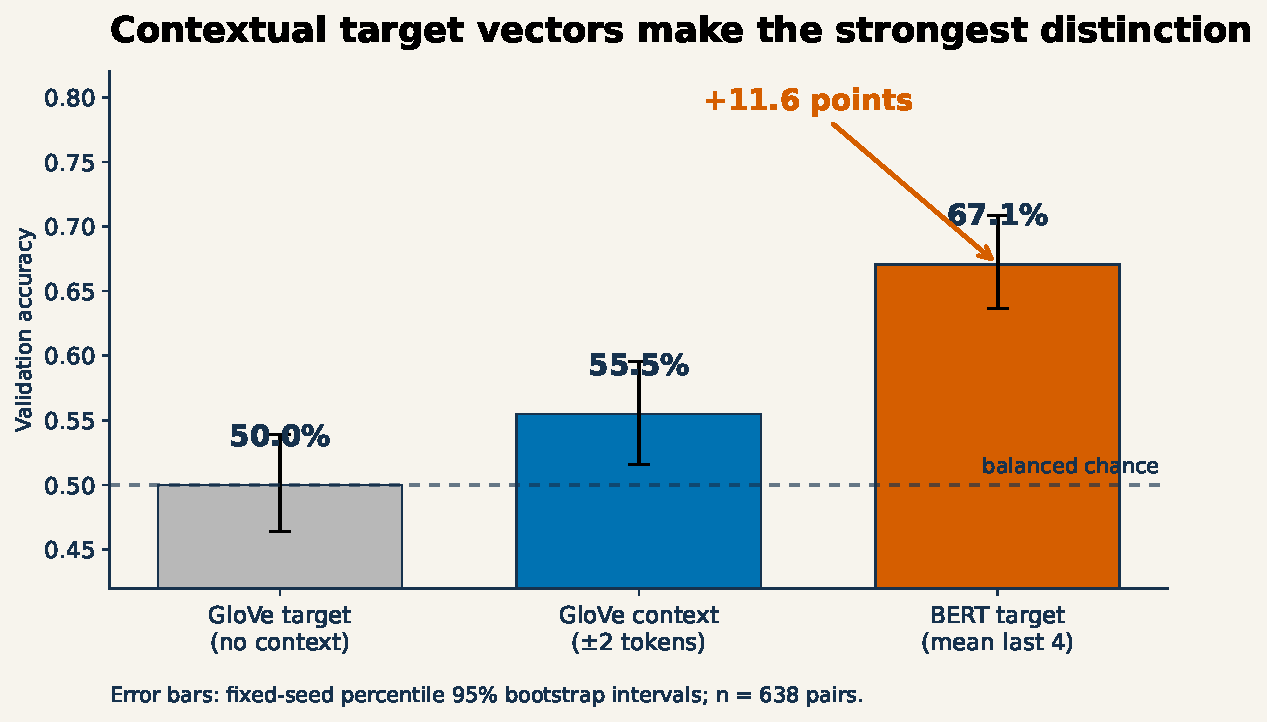
\includegraphics[width=\linewidth]{../figures/model_comparison.pdf}
\captionfont\RaggedRight
BERT reaches \BertAccuracy{} accuracy and \BertMacroF{} macro F1. The target-only
diagnostic is exactly constant; nearby static context restores limited signal.
\end{panel}

\begin{panel}{Same-sense scores separate more clearly}
\centering
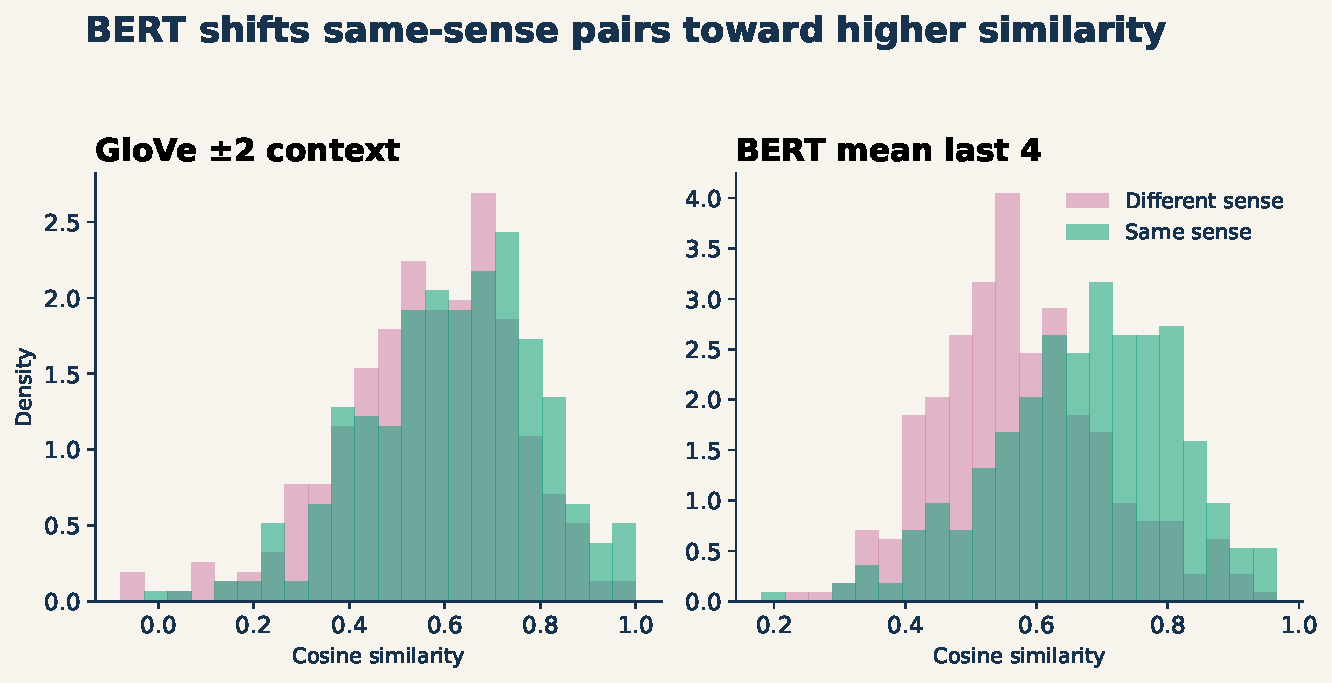
\includegraphics[width=\linewidth]{../figures/similarity_distributions.pdf}
\captionfont\RaggedRight
GloVe's label distributions overlap heavily. BERT shifts same-sense pairs toward
higher similarity, while substantial overlap remains (ROC-AUC 0.716).
\end{panel}

\begin{panel}{Paired evidence, not decorative error bars}
The BERT-minus-context gain is 74 additional correct pairs. In 1,000 paired
bootstrap resamples, the reverse contrast (GloVe minus BERT) remains below zero:
accuracy [\DifferenceLower{}, \DifferenceUpper{}] points and macro F1
[-16.9, -6.6] points.
\end{panel}

\begin{panel}{The systems fail in opposite directions}
BERT recovers 77.4\% of same-sense pairs but 56.7\% of different-sense pairs.
GloVe context recovers 46.4\% and 64.6\%, respectively. These class skews are
thresholded observations, not intrinsic representation preferences.
\end{panel}
\end{minipage}\hfill
\begin{minipage}[t]{0.316\textwidth}
\RaggedRight
\begin{panel}{Where the signal appears}
\centering
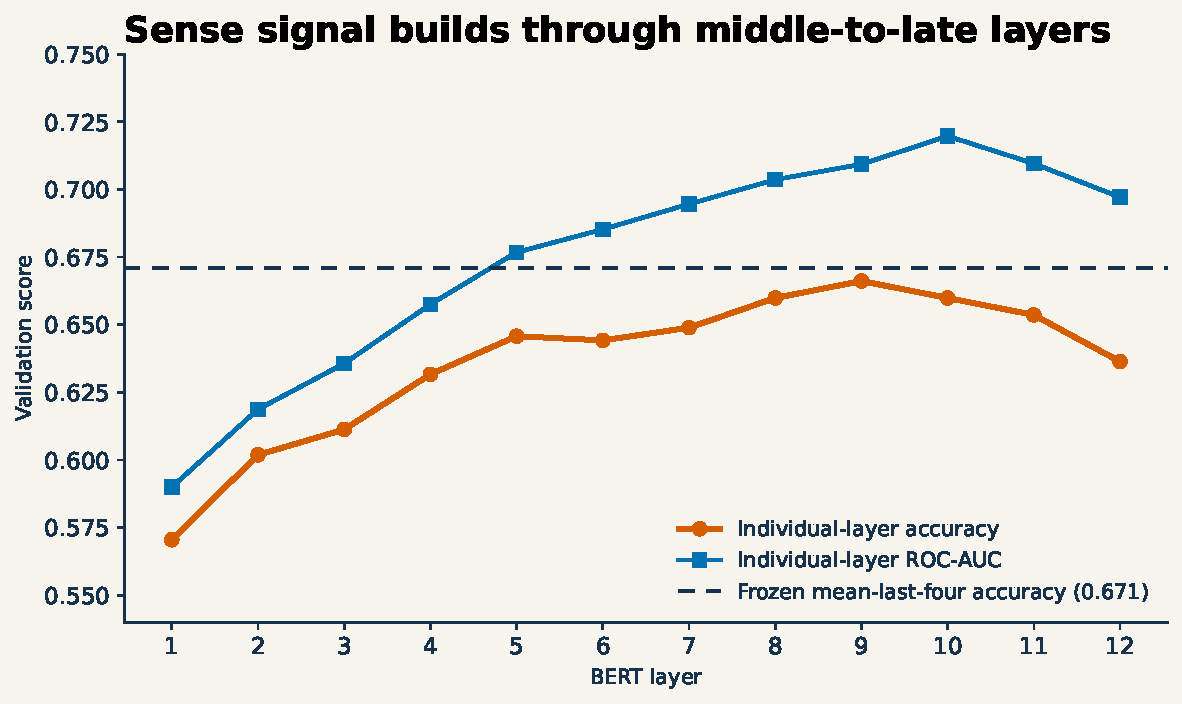
\includegraphics[width=\linewidth]{../figures/layer_analysis.pdf}
\captionfont\RaggedRight
Individual-layer accuracy rises broadly through layer 9 and falls at layer 12.
This is secondary validation analysis; it did not redefine the frozen primary
representation.
\end{panel}

\begin{panel}{One success, one warning}
\centering
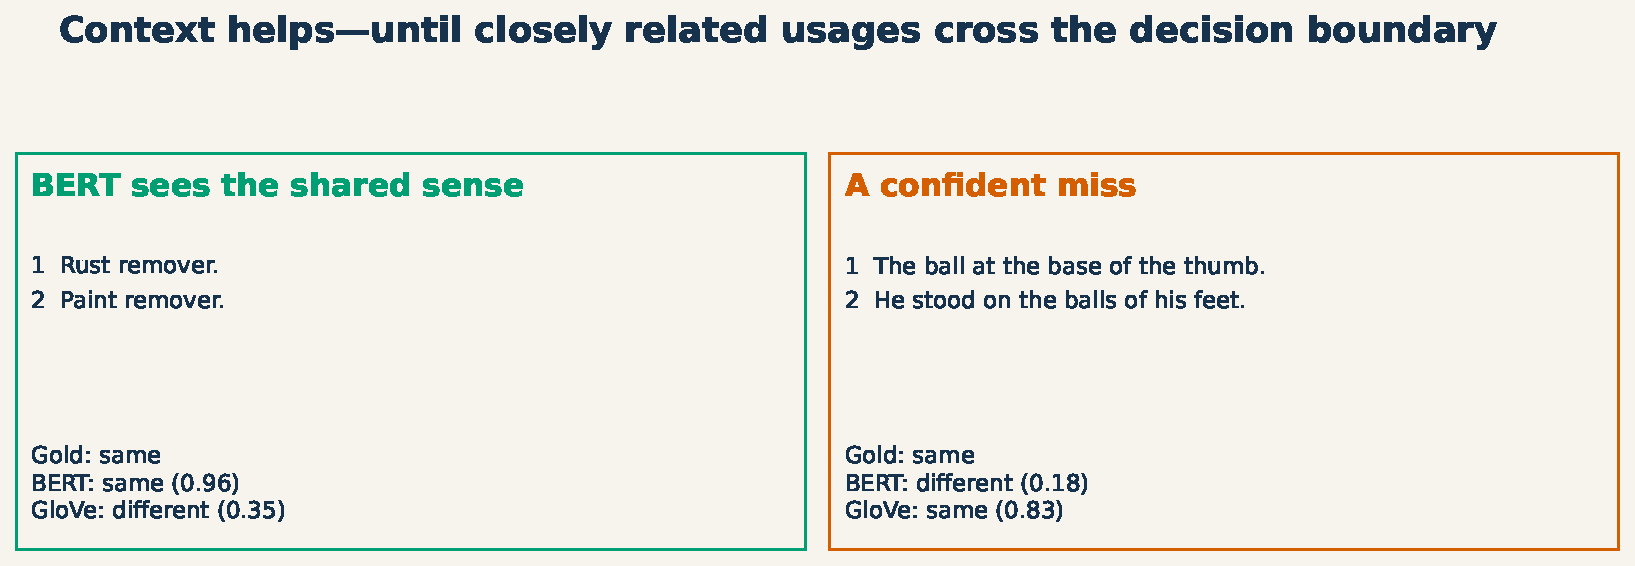
\includegraphics[width=\linewidth]{../figures/qualitative_cases.pdf}
\captionfont\RaggedRight
BERT is uniquely correct on \BertOnlyCount{} pairs; GloVe context is uniquely
correct on \StaticOnlyCount{}. A contextual representation improves separation,
but it does not settle fine-grained sense boundaries.
\end{panel}

\begin{panel}{Limitations}
\begin{itemize}\setlength\itemsep{2mm}
\item One balanced English benchmark and 638 validation pairs.
\item Frozen BERT features, not fine-tuning or a modern encoder comparison.
\item GloVe context is an unweighted lexical mean; syntax is absent.
\item Thresholded cosine tests geometry, not every fact encoded in a vector.
\item \BertErrorCount{} BERT errors remain; selected cases suggest hypotheses,
not causal explanations.
\end{itemize}
\end{panel}

\begin{panel}{Conclusion}
\key{Contextualization matters here.} Under one locked protocol, BERT target
vectors discriminate word meaning substantially better than local static context.
The middle-to-late layer pattern and confident errors also show that ``more
contextual'' is not the same as ``ambiguity solved.''
\end{panel}
\end{minipage}

\vfill
{\tinyfooter
\textbf{Sources:} [1] Pilehvar \& Camacho-Collados (2019), WiC,
doi:10.18653/v1/N19-1128. [2] Pennington et al. (2014), GloVe,
doi:10.3115/v1/D14-1162. [3] Devlin et al. (2019), BERT,
doi:10.18653/v1/N19-1423. [4] Loureiro et al. (2021), contextual WSD analysis,
doi:10.1162/coli\_a\_00405. Full methods, tables, references, and integrity
placeholder are in the appendix. Repository: \textbf{URL not supplied}.}
\end{document}
